\chapter{The FACT Open Crab Sample}
%
This analysis is exclusively using openly accessible data \cite{fact-data}. In November 2017 the
FACT collaboration made a dataset of Crab Nebula observations public
\cite{FACT-Design, FACT-Calib}. This dataset contains $\SI{17.7}{\hour}$
of Crab Nebula observations made between November 1, 2013 and November 6, 2013.
This sample is chosen because of the good observation conditions. Alongside the
data Monte Carlo simulations (MC) for diffuse proton air-showers and point-like
as well as diffuse gamma ray air-showers are distributed. The observations
cover a zenith distance between $\SIrange{6}{30}{\degree}$, \autoref{fig:zenith}.
%
\begin{figure}
  \centering%
  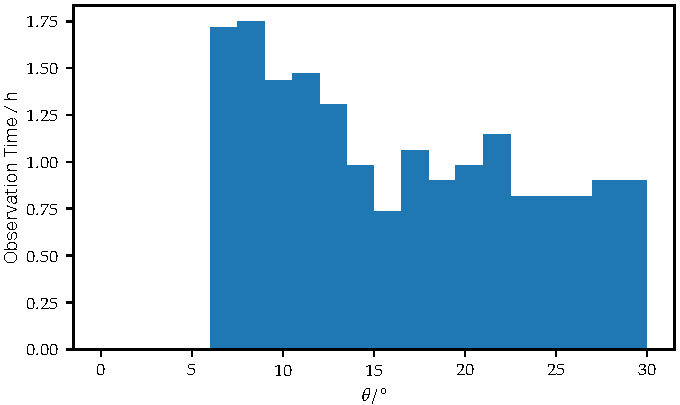
\includegraphics[width=0.8\textwidth]{Plots/zenith.pdf}%
  \caption{The distribution of the $\SI{17.7}{\hour}$ of Crab observations within the FACT open data sample over the zenith distance.}%
  \label{fig:zenith}%
\end{figure}
%
The simulated data represents Monte Carlo simulations of air-showers
originating from protons and photons. The data sets contain events from
simulated point sources and diffuse background sources. To train the analysis
tools, dedicated truths for each of the tasks are needed. The simulations
contain these truths, and are used for this task. Therefore, the quality of
these simulations is essential to the quality of the analysis. The simulations
are processed in two steps: firstly the interactions of cosmic rays with earths
atmosphere is computed and secondly, the interaction of the generated Cherenkov
light with the telescopes hardware is simulated. The first step is done by the
framework CORSIKA [cite]. The detector response of FACT's camera, including
triggers, is then determined for the simulated events using CERES [cite]. The
parameters used for generating the simulations are shown below.

\begin{table}
  \centering%
  \begin{tabular}{l
                  c
                  c}
      \toprule
      {}    & Gammas  & Protons      \\
      \midrule
      Energy Range & \SI{200}{\GeV} – \SI{50}{\TeV} & \SI{100}{\GeV} – \SI{200}{\TeV} \\
      Spectral Slope & \num{-2.7} & \num{-2.7} \\
      Max. Impact & \SI{270}{\meter} & \SI{400}{\meter} \\
      Zenith Distance & \ang{0} – \ang{30} & \ang{0} – \ang{30} \\
      CORSIKA Events & \num{12000000} & \num{780046520}\\
      Triggered Events & \num{1914812} & \num{509652}\\
      \bottomrule
  \end{tabular}
  \caption{Parameters and number of events regarding the MC simulated events.}
  \label{tab:mcs}
\end{table}
